\chapter{Implementación}\label{implementacion}

\section{Arquitectura del sistema}
Si bien el objetivo principal de este trabajo es incrementar la cobertura de Quepy, deseamos también que el sistema esté compartimentado de tal forma que sus componentes puedan utilizarse individualmente para otras aplicaciones.

La arquitectura de nuestro sistema integra tres grandes bloques que interactúan a través de interfaces:

\begin{description}
    \item[FeatMultinomialNB] Es el clasificador del sistema. Hereda del clasificador multinomial bayesiano \textit{MultinomialNB} de la librería scikit-learn (\citet{scikit-learn}) y está adaptado para soportar el entrenamiento utilizando tanto instancias como características. Elegimos este clasificador siguiendo a \citet{dualist}.
    \item[ActivePipeline] Es una clase que abstrae los ciclos de aprendizaje activo. Recordemos que constan de dos pasos principales donde se seleccionan las instancias o características y luego se procesan las etiqueta devueltas por el usuario. Para llevar a cabo estas tareas el ActivePipeline necesita tener acceso a los corpus etiquetados y no etiquetados y al clasificador, lo cual lo convierte en el módulo central del proyecto.
    \item[Preprocess] Es un módulo que convierte las preguntas de entrenamiento etiquetadas a su representación vectorial utilizando las características descriptas en el capítulo anterior. La representación de las preguntas está completamente ligada a los patrones de la aplicación de Quepy. Por ello diseñamos el preproceso como una extensión opcional de Quepy que puede utilizar cualquier clasificador. En otras palabras, no es necesario que se integre con el aprendizaje activo.
\end{description}

\subsection{ActivePipeline: Un marco de trabajo de aprendizaje activo sobre características e instancias}

ActivePipeline es una clase creada para simplificar la tarea del aprendizaje activo. Entre las actividades que realiza se encuentra la lectura de los conjuntos de datos, la selección de instancias y características para presentar al oráculo humano, la gestión de los datos ingresados y el reentrenamiento del clasificador. También agregamos funciones que facilitan el entorno de experimentación como sesiones y métricas de evaluación parcial.

Hasta el momento hemos realizado una prueba de concepto que demuestra que una aproximación de este estilo ayudaría a resolver el problema de la falta de cobertura de Quepy. Esta arquitectura está en desarrollo constante y no ha sido terminada para integrarse en un sistema estable para interactuar con un sistema real. Describiremos a continuación los puntos más centrales de la implementación ya que los detalles son altamente propensos a ser modificados en el futuro.

Para crear una instancia de ActivePipeline se requiere un diccionario con los siguientes parámetros:
\begin{description}
    \item[Clasificador] Es una instancia entrenable de un clasificador. Para mantener generalidad, requerimos que tenga la interfaz estándar de \textit{scikit-learn}. Los métodos que utilizamos son \textit{fit} para contruir el modelo a partir de los datos anotados, \textit{predict\_proba}, \textit{predict\_log\_proba} para obtener la probabilidad de cada clase dado un conjunto de instancias y \textit{score} que calcula el rendimiento del clasificador.
    \item[Conjuntos de datos] Se deben definir los archivos desde donde recuperar al menos tres conjuntos de datos: el de entrenamiento, el de evaluación y el no etiquetado. Ya deben estar preprocesados antes de ser leídos por el ActivePipeline, y es recomendable que sean instancias de una clase Corpus también definida en el sistema.
\end{description}

Al permitir elegir tanto características como el conjunto de datos y el clasificador, la clase ActivePipeline puede ser utilizada dentro de cualquier ámbito de aprendizaje activo incluso no relacionado al procesamiento del lenguaje natural.

Tanto para el aprendizaje sobre características y sobre instancias el ActivePipeline cuenta con una función automática. El usuario debe definir sólo las funciones de interacción con el usuario, es decir, cómo mostrar la información, y pasarlas como parámetros al ActivePipeline.

\subsection{FeatMultinomialNB: Un clasificador entrenado con características}

Como ya mencionamos anteriormente FeatMultinomialNB es un clasificador bayesiano ingenuo. Profundizaremos ahora en el fundamente teórico detrás de él y en las modificaciones que realizamos para soportar el entrenamiento con características.

Un clasificador bayesiano, explica \citet{libro-abney}, es un ejemplo de un modelo generativo. Estos modelos usualmente utilizan la distribución anterior de las clases $P(c)$ y la distribución de las instancias específica para la clase o verosimilitud $P(x|y)$. Su nombre se debe a que un modelo es una hipótesis acerca de cómo cada instancia puede ser generada por una clase. Se utiliza esta probabilidad generativa para la clasificación a través del teorema de Bayes:

$$P(x|c) = \frac{P(c)P(x|y)}{P(x)}$$

El \textit{MultinomialNB} descripto por \citet{multinomial-manning} se basa en la asunción ingenua de que el valor de cada una de las características de una instancia es independiente de las demás. Si bien sabemos que esto no es así y que cada característica sí se relaciona con las restantes, este clasificador es ampliamente utilizado para la categorización de texto \citet{dualist}, \citet{multinomialnb-comparision-mccallum} y \citet{multinomialnb-unbalanced}. Su principal ventaja es la simplicidad, lo que en nuestro caso ayudó a su adaptación para esta tarea de aprendizaje activo.

En gran parte de la bibliografía se asume que las características de una instancia serán sólo las palabras presentes en el documento o instancia, lo cual no se ajusta a la representación elegida para este problema. Por lo tanto, hemos cambiado levemente la notación que utilizan otros autores reemplazando palabras como \textit{words} o \textit{terms} por \textit{características}. También hemos reemplazado \textit{documents} por \textit{instancias}.

Bajo este modelo, la probabilidad de que una instancia $x_i$ sea de clase $c_j$ es computada utilizando la fórmula:
\begin{equation}\label{eq-mnb-prob}
    P(c_j|x_i) \propto P(c_j) \prod_{1\leq k \leq n_i}P(f_k|c_j)
\end{equation}
donde $n_i$ es la cantidad de características que aparecen en la instancia $x_i$ y $P(f_k|c_j)$ es la probabilidad de que la característica $f_k$ esté presente en una instancia de clase $c_j$. \citet{multinomial-manning} explican que la intuición detrás de estos conceptos es que $P(f_k|c_j)$ indica de qué tan buen indicador es $f_k$ para la clase $c_j$, mientras que $P(c_j)$ pesa estos valores por la probabilidad de la clase. El producto de las probabilidades y pesos es una medida de cuánta evidencia existe de que la instancia pertenezca a la clase.

La gran cantidad de multiplicaciones sobre valores probabilísticos menores que uno puede llevar fácilmente a un desbordamiento aritmético debido la imposibilidad de representar números tan pequeños en una computadora. Utilizaremos logaritmos para manejar esta situación, manteniendo la proporción de los operandos ya que el logaritmo es una función monótona creciente y basándonos fuertemente en la propiedad que asegura $\log(ab) = \log(a) + \log(b)$. La ecuación \ref{eq-mnb-prob} es equivalente a:

\begin{equation}
\log P(c_j|x_i) \propto \log P(c_j) + \sum_{1\leq k \leq n_i} \log P(f_k|c_j)
\end{equation}

La tarea de clasificación se reduce entonces a encontrar la clase $c_j$ que maximice la ecuación \ref{eq-mnb-prob}. Volviendo a la definición \ref{def-clasificacion}, podemos reescribirla como:

\begin{definition}
\begin{equation}
    \Phi(x_i) = \operatorname*{argmax}_{c_j \, \in \, \mathcal{C}} \; \log P(c_j|x_i) = \operatorname*{argmax}_{c_j \, \in \, \mathcal{C}} \; \log P(c_j) + \sum_{1\leq k \leq n_i} \log P(f_k|c_j)
\end{equation}
\end{definition}

Nuestro modelo depende entonces de dos parámetros: $P(c_j)$ y $P(f_k|c_j)$. Sin embargo no conocemos las distribuciones reales de estas variables, y por lo tanto las estimaremos empíricamente a partir de los datos observados. Existen muchas formas de obtener estos parámetros, la que proponemos a continuación es un ejemplo de un entrenamiento supervisado ya que utiliza instancias etiquetadas. Llamaremos $\hat{P}(c_j)$ y $\hat{P}(f_k|c_j)$ a las estimaciones respectivamente, que se calculan utilizando estimadores de máxima verosimilitud:

\begin{equation}
\hat{P}(c_j) = \frac{\sum_{x \in \mathcal{L}} \, \hat{\Psi}(x, c_j)}{|\mathcal{L}|}
\end{equation}
\begin{equation}\label{sin-smooth}
\hat{P}(f_k|c_j) = \frac{\sum_{x \in \mathcal{L}} \, \hat{\Psi}(x, c_j) f_k(x)}{\sum_{x \in \mathcal{L}} \, f_k(x)}
\end{equation}

donde $\mathcal{L}$ es el conjunto de datos etiquetados de entrenamiento, $\hat{\Psi}(x, c_j) \in \{0,1\}$ es la clasificación obtenida del mismo y $f_k(x)$ es la cantidad de veces que la característica $f_k$ está presente en la instancia $x$.

Aunque las ecuaciones están bien definidas, puede suceder que el numerador de la ecuación \ref{sin-smooth} $\sum_{x \in \mathcal{L}} \hat{\Psi}(x, c_j) f_k(x)$ sea nulo ya que una característica puede no ocurrir en ninguna instancia de la clase. Debido a la raleza en la distribución de palabras (\citet{zipf1} y \citet{zipf2}), es común que ocurra este fenómeno. Para evitarlo se suavizan los datos de la siguiente manera:

\begin{equation}
\hat{P}(f_k|c_j) = \frac{m_{jk} + \sum_{x \in \mathcal{L}} \hat{\Psi}(x, c_j) f_k(x)}{\sum_{x \in \mathcal{L}} (f_k(x) + m_k)}
\end{equation}

\citet{dualist} plantea que $m_{jk}$ es la probabilidad anterior o a priori de $f_k$ para la clase $c_j$, es decir, una cantidad desconocida que expresa la incertidumbre acerca de la distribución de probabilidad de las características. Al ser desconocida comúnmente se utiliza en su lugar una distribución uniforme como la Laplaciana donde todos los valores son 1. El término $m_k$ es un valor para normalizar la división.

Nuestro objetivo principal es poder entrenar el clasificador con información sobre la relación entre las características y las clases. Adaptamos entonces el \textit{MultinomialNB} para que utilice un parámetro adicional $m_{jk}$ modificando esta probabilidad anterior siguiendo las etiquetas de las características que provee oráculo humano. Introduciremos entonces la siguiente definición:

\begin{definition}
La clasificación de una características es una función $\Psi_f:\mathcal{F} \times \mathcal{C} \rightarrow \{0, 1\}$ que asigna valores booleanos donde $\mathcal{F}$ es el conjunto de características y $\mathcal{C}$ es el conjunto de clases posibles.
\end{definition}

Seguimos la implementación de Dualist para agregar esta clasificación adicional de la siguiente manera:

\begin{equation}\label{eq-feat-boost}
m_{jk} = 1 + \Psi_f(f_k, c_j) \; \alpha
\end{equation}

donde $\alpha$ es una constante y $\Psi_f$ es la clasificación aprendida del usuario.

\vspace{5 mm}
En las secciones siguientes describiremos cómo implementamos algunos módulos que intervienen en el aprendizaje activo. En la figura \ref{aa-con-secciones} se ilustran en qué momento del ciclo se utilizan estas implementaciones.

\begin{figure}[h!]\label{aa-con-secciones}
\centering
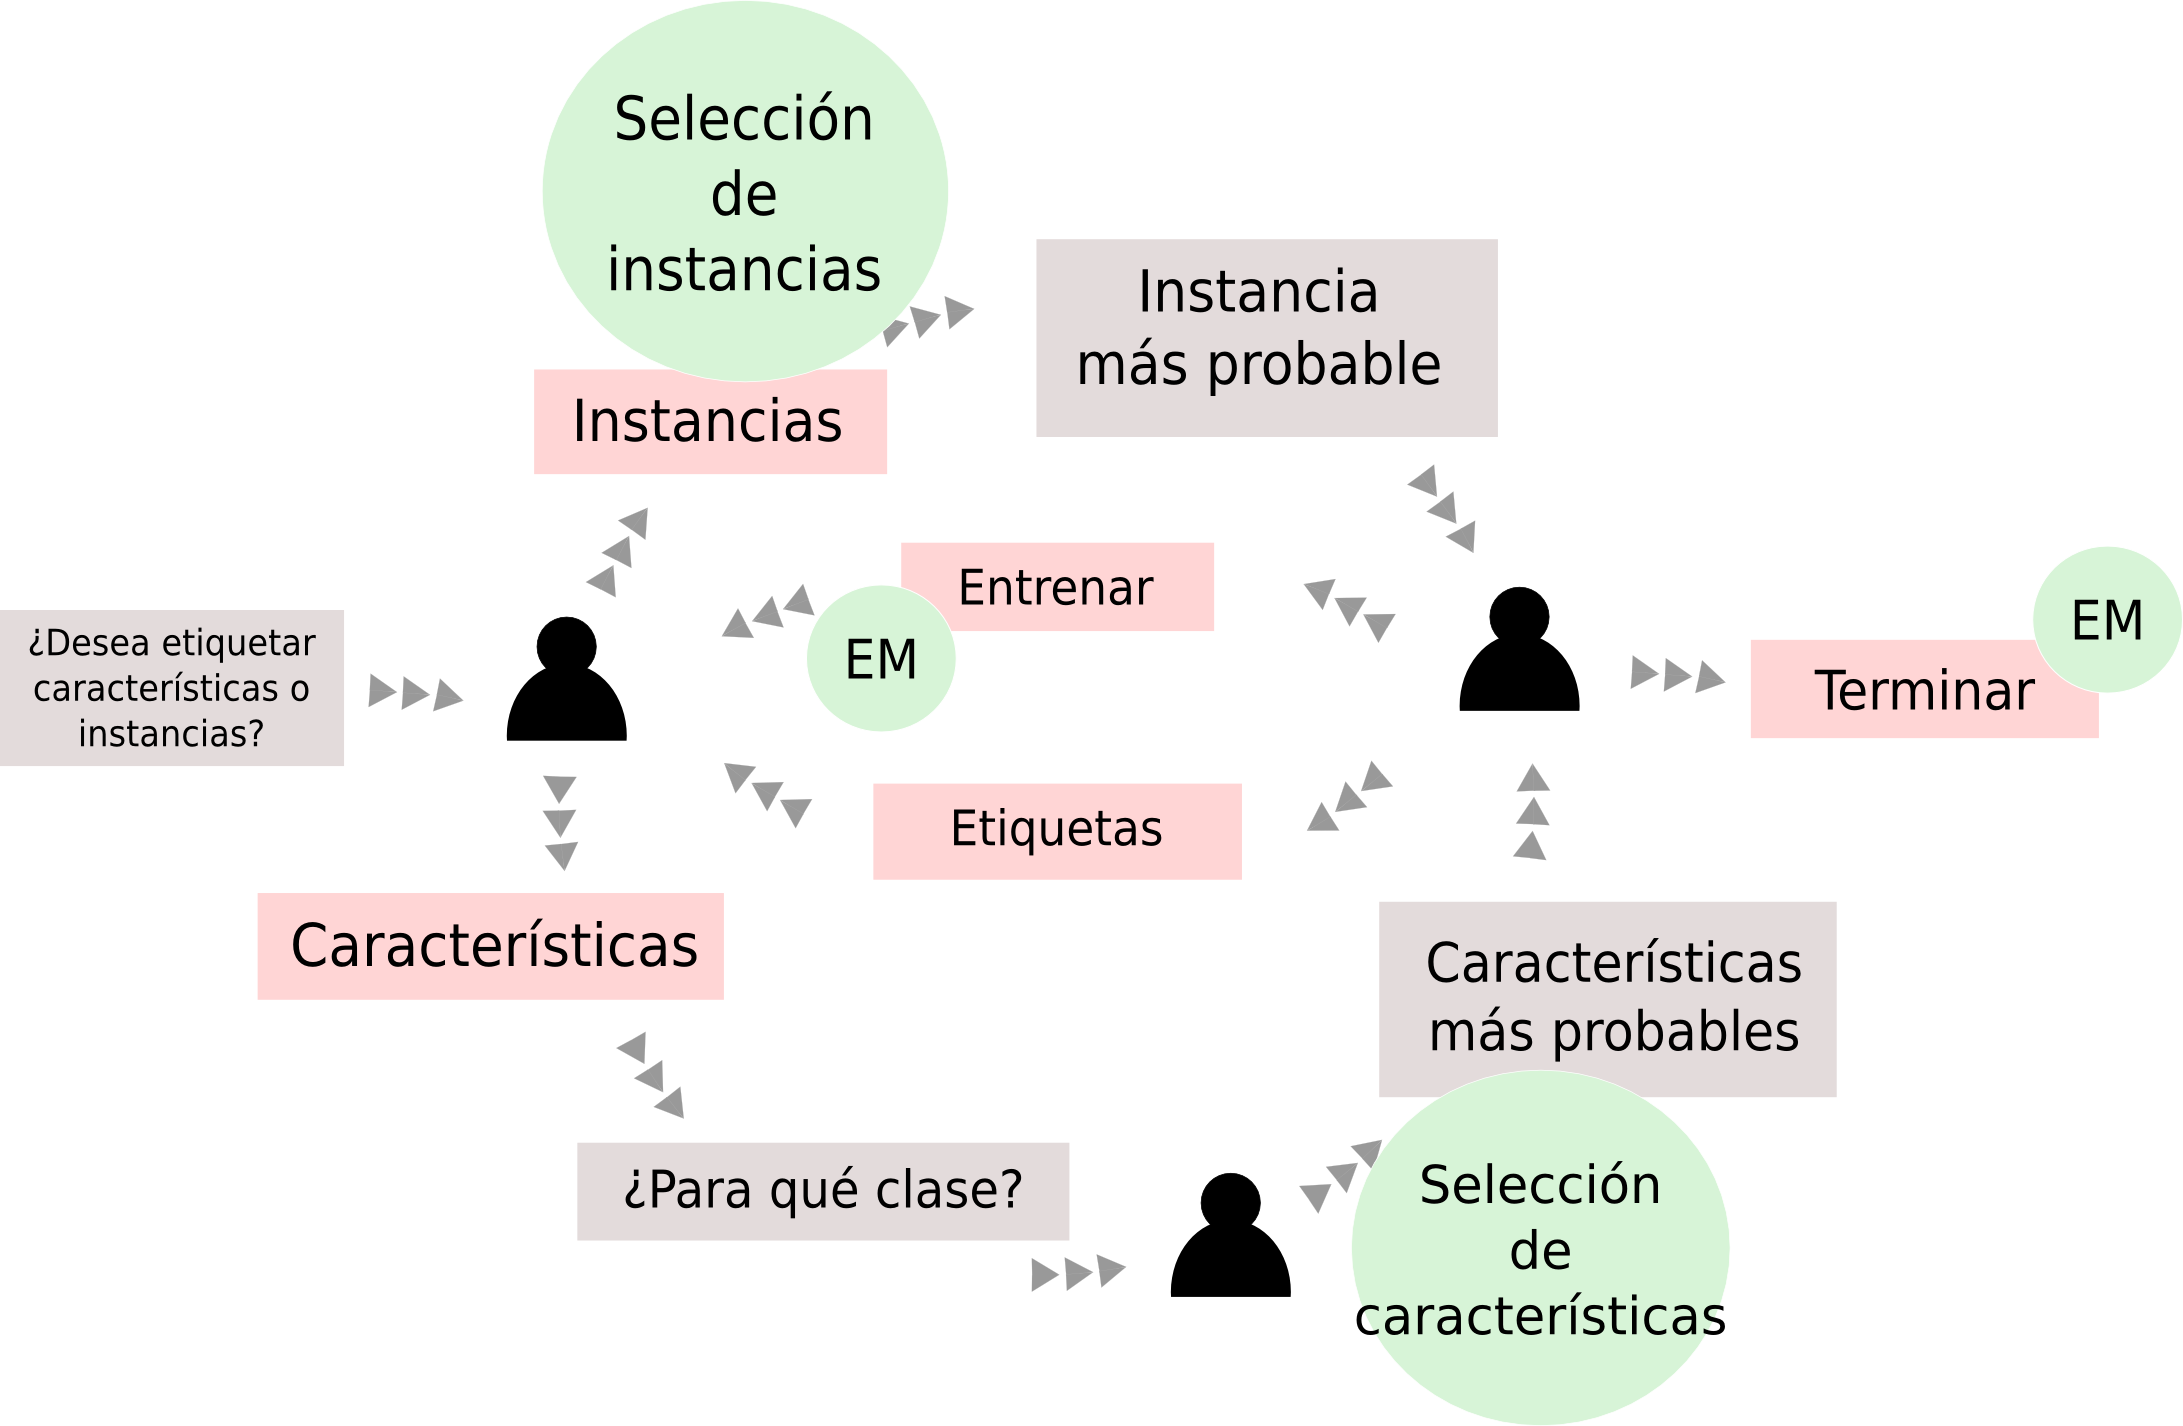
\includegraphics[width=10cm]{partes-implementacion}
\caption{Diagrama de la implementación del sistema aprendizaje activo.}\label{aa-con-secciones}
\end{figure}

\section{Selección de instancias}

Elegir las instancias para que sean etiquetadas por el usuario es central en los algoritmos de aprendizaje activo y existen numerosas estrategias que pueden utilizarse. Trabajos como \citet{settles_active_learning_survey} y \citet{al-logistic-regresion-schein} resumen las más importantes de ellas:

\begin{description}
    \item[Muestreo por incertidumbre] Asumiendo que el aprendedor tiene cierto     grado de certidumbre a la hora de etiquetar un ejemplo, hay varias formas     de utilizar esta información para seleccionar los ejemplos que se enviarán     al oráculo:
    \begin{itemize}
        \item Confianza o incertidumbre en su clasificación.
        \item Distancia entre la dos primeras etiquetas más probables.
        \item Entropía.
    \end{itemize}
    Algunos estudios han mostrado que dichas estrategias obtienen resultados similares y que la elección debe hacerse teniendo en cuenta la aplicación particular para la que se utilizarán.
    \item[Selección por comité (QBC)] Se utilizan varios clasificadores para obtener
    un conjunto de etiquetas para cada una de las instancias no etiquetadas.
    Luego se seleccionan las instancias que hayan generado mayor desacuerdo
    entre los clasificadores.
    \item[Cambio esperado del modelo] Selecciona las instancias que generarían
    un mayor cambio en el modelo (aprendedor) si se supiera su etiqueta. Como
    medida de cambio se utiliza el largo del gradiente del modelo (EGL). Se ha
    demostrado que funciona bien empíricamente, pero puede ser
    computacionalmente caro.
    \item[Reducción del error esperado] Es similar al método anterior, pero en
    lugar de maximizar el cambio en el modelo, minimiza su error de
    generalización. El objetivo es reducir el número esperado de predicciones
    erróneas. Este método ha sido ampliamente estudiado demostrando muy buenos
    resultados. Sin embargo, es el método computacionalmente más costoso.
    \item[Reducción de la varianza] Intenta minimizar el error esperado indirectamente minimizando la varianza de los resultados. Para ello, selecciona un conjunto de instancias que maximice la cantidad de información Fisher. Al igual que en el método anterior tiene en cuenta todo el espacio de ejemplos en lugar de cada una de las instancias, y por lo tanto tiene menos probabilidades de seleccionar ejemplos raros en la distribución.
    \item[Métodos pesados por la densidad] Siguiendo la misma línea que los dos
    métodos anteriores, supone que los ejemplos significativos son aquellos
    que no solo tienen alta incertidumbre, sino que son representativos
    de la distribución subyacente. Algunos estudios indican resultados superiores,
    acompañados por implementaciones de alta velocidad que permiten incluso
    interacción de tiempo real con el usuario.
\end{description}

De todas estas opciones elegimos explorar el espacio de instancias a través de la entropía definida por \citet{entropy-shannon} como:
\begin{equation*}
\mathcal{H}(x) = - \sum_{c_i\,\in\,\mathcal{C}} \, P(c_i|x)\; \log\,P(c_i|x)
\end{equation*}
\citet{information-theory-cover} explica en términos simples que la entropía es la cantidad de información necesaria para representar una variable aleatoria. \citet{multinomial-manning} plantea también que la entropía es una forma de medir la incertidumbre, ya que se maximiza cuando las etiquetas para una instancia son equiprobales y se vuelve 0 cuando la instancia está etiquetada.

Este método ha sido utilizado previamente como parte del aprendizaje activo por \citet{entropy-or}, \citet{settles-entropy} y \citet{Hwa-entropy}. Nosotros lo tomamos por varios motivos:
\begin{itemize}
    \item Es simple y rápido de calcular.
    \item Tiene en cuenta la incertidumbre de todas las clases, no sólo una o dos de ellas.
    \item \citet{settles_active_learning_survey} sostiene que la entropía es más adecuada cuando se busca minimizar la pérdida o \textit{log-loss}, definida como la desviación de la clasificación; mientras que los otros métodos son adecuados para minimizar el error. En particular buscamos que el clasificador se desempeñe correctamente en todas las clases y no sólo en la clase mayoritaria.
\end{itemize}


% In the case of uncertainty sampling using the Shannon entropy measure of uncertainty, bad performance goes hand by hand with noise, as defined by the portion of squared error that is training set size independent. For margin sampling, inability to identify the pairs of categories forming the margin on multi-category problems is the biggest danger, as seen on the NewsGroups data set. In spite of this observation, margin sampling competes favorably with the alternative heurstics and is the most computationally efficient method examined.

\section{Selección de características}\label{instance-selection}

Un criterio ampliamente utilizado para la selección de características es la Ganancia de Información o \textit{Information Gain}. Algunos estudios que destacan su uso como medida de relevancia son \citet{dualist}, \citet{forman-ig} y \citet{Sebastiani-text-categorization}

\citet{infgain} define la ganancia de información como la cantidad de información en bits sobre la predicción de la clase, si la única información disponible es la presencia de la característica y la distribución de la clase correspondiente. En otras palabras, mide la reducción esperada de la entropía cuando la característica está presente o ausente. Podemos expresarla según la siguiente fórmula:

\begin{equation}
\mathcal{IG}(\mathcal{X}, \mathcal{Y}) = \mathcal{H}(\mathcal{X}) - \mathcal{H}(\mathcal{X}|\mathcal{Y}) = \mathcal{H}(\mathcal{Y}) - \mathcal{H}(\mathcal{Y}|\mathcal{X})
\end{equation}

Notemos que es una función entre variables aleatorias, donde una es la presencia de una característica y otra es la clase. Para la clasificación de texto en particular, podemos reemplazar la fórmula de la entropía y definir la ganancia de información como:

\begin{equation}
\mathcal{IG}(f_k) = \sum_{I_k} \sum_j P(I_k, c_j)\,\log \frac{P(I_k,c_j)}{P(I_k)P(c_j)}
\end{equation}

donde $I_k \in \{0, 1\}$ indica la presencia o ausencia de la característica k.

Algunas de estas probabilidades no son parte del modelo, por lo que las estimamos empíricamente como:
$$ \hat{P}(I_k = 1) = \frac{|\{ x \in \mathcal{X}: f_k(x) > 0 \} |}{|\mathcal{X}|} $$
$$ \hat{P}(I_k = z, c_j) = \frac{|\{ x \in \mathcal{X}: I_k(x) = z \wedge \Psi(x, c_j)\} |}{|\mathcal{X}|} $$
$$ \hat{P}(I_k = 0) = 1 - \hat{P}(I_k = 1) $$
donde $\mathcal{X}$ es el conjunto de instancias.

Para simplificar la tarea de etiquetamiento, presentamos al usuario las características asociadas a las clases para las que son más probables. Esta selección se realiza en dos pasos: primero seleccionamos las k características que coocurren más veces con la clase y luego las ordenamos por su ganancia de información.

\section{Esperanza-Maximización}
El algoritmo de esperanza-maximización propuesto por \citet{Dempster-maximumlikelihood} es ampliamente utilizado para inferir parámetros desconocidos en una distribución que tiene estados latentes. Para la clasificación de texto, los estados latentes son las clases de las instancias.

Esperanza-Maximización es utilizado como un método de entrenamiento de clasificadores no supervisado, es decir, con datos no etiquetados. La variante que propone \citet{dualist} y que describiremos a continuación incluye tantos instancias etiquetadas como no etiquetadas. El objetivo de aplicar este algoritmo es introducir al clasificador parte de la información de los datos no etiquetados al maximizar la probabilidad de los datos observados.

Ya hemos definido previamente el concepto de verosimilitud o \textit{likelihood} del modelo: es una función sobre los parámetros del modelo y un conjunto de datos que calcula la probabilidad de los valores tomados por cada variable aleatoria del modelo bajo dichos parámetros. Podemos escribirlo como:

\begin{equation}
L(\theta) = P(\mathcal{X}_l, \mathcal{C}_l; \theta)
\end{equation}

donde $\theta$ representa a los parámetros y $\mathcal{L} = (\mathcal{X}_l, \mathcal{C}_l)$. Como las instancias de entrenamiento se asume que son independientes e idénticamente distribuidos, entonces podemos escribir las dos siguientes fórmulas equivalentes:

\begin{equation}
L(\theta) = \prod_{x_i, c_i \in \mathcal{L}} P(x_i, c_i; \theta)
\end{equation}
\begin{equation}
l(\theta) = \log L(\theta) = \sum_{x_i, c_i \in \mathcal{L}} \log P(x_i, c_i; \theta)
\end{equation}

Si llamamos $cant(c_j)$ a la cantidad de instancias etiquetadas con la clase $c_j$, entonces definimos:

\begin{equation}
l(\theta) = \sum_{x_i \in \mathcal{L}, \, c_j \in \mathcal{C}} cant(c_j) \log P(x_i, c_j; \theta)
\end{equation}

\begin{equation}\label{loglikelihood}
l(\theta) = |\mathcal{X}_l| \sum_{x_i \in \mathcal{L}, \, c_j \in \mathcal{C}} P(c_j) \log P(x_i, c_j; \theta)
\end{equation}

A grandes rasgos, el algoritmo funciona en dos pasos E y M, por sus siglas en inglés \textit{Expectation} y \textit{Maximization}.

El paso E es el que calcula el valor esperado de la verosimilitud asumiendo que la distribución actual es verdadera y no existen variables no observadas. Para realizarlo, utilizamos el clasificador en su estado actual para etiquetar probabilísticamente el conjunto de datos no etiquetados, y asumimos dichas etiquetas como correctas. Con este conjunto de nuevos datos se calcula el $l(\theta)$ del modelo según la ecuación \ref{loglikelihood}.

Si los parámetros actuales fueran correctos, entonces la verosimilitud obtenida sería la verosimilitud real del modelo, pero como no lo son provee una cota inferior. Luego, como tenemos una función sin valores no observados, el paso M maximiza $l(\theta)$ encontrando parámetros del modelo más adecuados. De esta forma optimizamos la cota inferior encontrada generando un nuevo conjunto de parámetros $\hat{\theta}$.

Ambos pasos se repiten numerosas veces hasta lograr convergencia. En nuestros experimentos, tomamos ejemplo de Settles, y realizamos una sola iteración, dado  que las siguientes iteraciones no aportan significativamente a la precisión del clasificador.

Si bien derivar la maximización correcta de los parámetros del $MultinomialNB$ no es trivial, la implementación posterior sí es sencilla. Para realizarlo nos basamos en la maximización de un clasificador Bayesiano simple de \citet{data-mining-Liu}, agregando la noción de \citet{dualist} de utilizar tanto los datos etiquetados como no etiquetados pesando los no etiquetados por un factor de 0,1.

Al etiquetar probabilísticamente los ejemplos no anotados con el clasificador se obtiene una matriz con $P(c_j|x_i)$ para cada instancia y cada clase. En base a ella y a los parámetros actuales del clasificador reestimamos los nuevos parámetros de la siguiente forma:

\begin{equation*}
\hat{P}_u(c_j) = \sum_{x_i \in \mathcal{U}} P(c_j|x_i) P(x_i)
\end{equation*}
\begin{equation*}
\hat{P}_u(f_k|c_j) = \sum_{x_i \in \mathcal{U}} P(c_j|x_i) P(x_i) f_k(x_i)
\end{equation*}

\begin{equation*}
\hat{P}_l(c_j) = \sum_{x_i \in \mathcal{U}} P(c_j|x_i) \Psi(x_i, c_j)
\end{equation*}
\begin{equation*}
\hat{P}_l(f_k|c_j) = \sum_{x_i \in \mathcal{U}} P(c_j|x_i) \Psi(x_i, c_j) f_k(x_i)
\end{equation*}

\begin{equation}
\hat{P}(c_j) = \frac{0.9 * \hat{P}_l(c_j) + 0.1 * \hat{P}_u(c_j)}{\mathcal{Z}_1}
\end{equation}
\begin{equation}
\hat{P}(f_k|c_j) = \frac{0.9 * \hat{P}_l(f_k|c_j) + 0.1 * \hat{P}_u(f_k|c_j)}{\mathcal{Z}_2}
\end{equation}

donde $\mathcal{U}$ es el conjunto de datos no etiquetados y $\mathcal{Z}_1$, $\mathcal{Z}_2$ son contantes de normalización.
